\documentclass[12pt]{article}
\usepackage{graphicx}
\usepackage{caption}
\usepackage{natbib}
\usepackage{authblk}
\usepackage[T1]{fontenc}
\usepackage[utf8]{inputenc}
\usepackage{setspace}
\usepackage{gensymb}
\usepackage{rotating}
\usepackage[british]{datetime2}
\usepackage{relsize}
\usepackage{hyperref}
\usepackage[top=28truemm,bottom=26.5truemm,left=25.5truemm,right=25.5truemm]{geometry}

% Setting color for hyperlinks
\hypersetup{
	colorlinks=true,
	citecolor=black,
	urlcolor=blue,
}

% Fix issue with links in references
\renewcommand{\harvardurl}{\textbf{URL:} \url}

% Changing the format of the affiliation 
\renewcommand\Affilfont{\itshape\small}

% Front page
\title{Communal violence and the legacy of precolonial states}
\author[$\dagger$]{Marius Swane Wishman}
\author[$\ddagger$]{Ole Magnus Theisen}
\affil[$\dagger$]{Department of Sociology and Political Science, NTNU}
\affil[$\ddagger$]{Independent PhD researcher}

\date{\today}

\providecommand{\keywords}[1]
{
	\small	
	\textbf{\textit{Keywords---}} #1
}

\begin{document}

\maketitle

\begin{abstract}
	As you can tell this is a very early draft. Please do not distribute
	without the authors consent. We are looking forward to your comments and
	feedback.
\end{abstract}

\bigskip

\keywords{Precolonial states, communal violence, conflict, VIP presentation}

\pagebreak

\onehalfspacing

The level of violence in non-state societies is qualitatively different from
that within states with rates of violence often being several orders magnitude
higher in the former \citep{diamond2013world, LeBlanc2003, Pinker2012}. Part of
this can be explained by that states’ primary objective and defining
characteristic is to solve the security dilemma \citep{Hobbes, Lake_1996}.
Several states in contemporary sub-Saharan Africa are judicially effective, but
empirically less so \citep{Jackson_1982}. This has resulted in pockets where
resolution of violent conflicts is mainly left to local traditional mechanisms
without a neutral arbiter to mediate or enforce peace should things get out of
hand. There might be important variations in this semi-anarchic situation,
however, as some areas have a long precolonial legacy of statehood which
previously addressed the security dilemma between ethnic groups. Some claim that
the existence of precolonial states has caused legal ambiguities that are
important causes of intergroup violence \citep{Eck2014}, others hold that
remnants of precolonial institutions directly \citep{Herbst2014, Wig2018} or
indirectly reduce the overall number of inter-ethnic (non-state) conflicts. 

\section{How conflicts are prevented or resolved without the state}

In order to explain how areas where precolonial states existed reduce communal
violence today, we first outline mechanisms regulating inter-communal conflicts
in contexts of weak statehood, before we investigate how precolonial states
might moderate these. While the quantitative literature on communal violence has
focused much on the type of issues that can trigger conflict between groups
\citep{Doring2020, Eck2014, Elfversson2015, Fjelde2014, Fjelde2012,
Hillesund_2017, Theisen2012}, the theoretical literature preceding statistical
studies emphasized structural factors that affect the underlying rationale of
resolving disputes peacefully or not. A more systematic understanding of how the
history of statehood shapes such structural characteristics is therefore wanting
in the quantitative literature. 

With the lack of an overarching authority to arbitrate between groups or provide
physical security, strategic interaction between groups arises in which physical
security is paramount. Problems related to interpersonal crime or competition
over resources are ubiquitous both within and between groups, and while they
might be systematically related to the outbreak of communal violence, they often
seem quite banal.\footnote{Hence Roy's \citep[1]{roy1994some} seminal study's
	titled \textit{Some Trouble with Cows} starts with: `In a remote village
somewhere in South Asia, someone's cow ate someone else's crop. Within two days,
tens of thousands of men were ranged against each other...'.} Strategic
interactions make otherwise mundane problems of criminal punishment or competing
policy preferences potential triggers of intergroup violence
\citep{diamond2013world, Eaton_2008, Fearon1995, Fearon_1996, Lake_1996}. Since
conflict is costly, however, there should be a rational interest in a bargained
solution short of violence \citep{Fearon1995}, but the problem is, when
strategic dilemmas arise, such bargained solutions are hard to establish and
uphold. Three related phenomena –- information problems, commitment problems,
and the security dilemma –- are each sufficient in causing armed conflict, but
very frequently co-occur \citep[46]{Lake_1996}. While our contention is that
states reduce these, we first present them separately.

\subsection{Problems with information, credible commitments, and the security
	dilemma} While dense networks within ethnic groups facilitate
	information exchange in turn preventing opportunistic behaviour as
	individuals can be identified and punished, in cross-ethnic
	interactions, identifying individuals is often much harder due to less
	frequent interactions, thinner networks, and cultural differences making
	it harder to identify opportunists
	\citep[719]{Fearon_1996}.\footnote{This should depend on the degree of
	interethnic interaction, which in turn can be facilitated by states –
see discussion below.} Consequently, individual punishment of noncoethnics is
difficult. Generally, information problems tend to grow more acute with
increasing state weakness \citep[46]{Fearon1995, Lake_1996}.

Relatedly, ethnic groups cannot credibly commit to mutually beneficial
agreements. At least they cannot be certain that other groups stay true to their
promises. Thus, the credibility of agreements between ethnic groups are often
premised on a supra-ethnic authority, and they are often initiated by the weaker
group that have most to fear from unregulated interaction (see below on
intragroup policing as an example)\citep[50]{Lake_1996}. In the absence of such
working arrangements, chronic insecurity about the other group’s intentions
ensues with conflict representing a realistic alternative \citep[51]{Lake_1996}.

The semi-anarchic situation found in areas where no supra-ethnic authority can
bind parties to their promises induces groups to apply self-help strategies. The
information problem renders groups chronically uncertain about others’ true
intentions, making defensive moves by one group look suspicious causing other
groups to safeguard themselves. While it may be collectively rational to reveal
private information to counterparts as part of a bargain to avoid conflict,
groups can have strategic incentives to withhold information, particularly if
revealing it make them vulnerable to an early confrontation from the other group
\footnote{For instance, \citet{Eaton_2008} notes that pastoral groups in East
	Africa are reluctant to invite members from adversaries to peace
negotiations in their territories as they may use the opportunity to scout for
future raids.} or make them more vulnerable in the future. This can cause
bargaining to crash and conflict to start as there might be a preference to
attack early rather than being victimized at a later occasion. Subsequently,
this makes all groups less safe, in particular when there are clear advantages
to use pre-emptive tactics\footnote{Since mobility increases the advantages of
	offensive relative to defensive tactics, one expectation could be that
	pastoralist groups whose livelihoods depend on mobility are more likely
	to resort to preemptive tactics and therefore see more violence in the
end.}, as Lake and Rotchild puts it ‘Fearful that the other might preempt, a
group has an incentive to strike first and negotiate later’
\citep[53]{Lake_1996}.

\subsection{Interethnic institutions that address the security dilemma}

Minor crimes or disagreements between individuals of different ethnic groups are
liable to trigger asymmetric reprisals by the victim’s group in which all
members of the perpetrator’s group are legitimate targets.\footnote{ Whether all
	member or e.g. all adult male relatives or some other collectively
derived criteria makes member of the perpetrator’s group legitimate targets
depends on the context, but secondary to our argument. The point is that
retribution is based on collective characteristics.} While likely triggering
escalatory cycles of counter-reprisals, the information-problem initially
prevents individual punishment of crimes, leaving the alternative to collective
retaliation to infringements by outsiders being no punishment at all. The fear
of collective retaliation must be sufficiently likely and brutal to deter,
making this mechanism of fear very vulnerable to minor incidents
\citep{Fearon_1996}. An earned reputation for ruthlessness, even in the face of
superior groups, can therefore work to uphold the peace, but only to a limited
extent [insert brief example from Omo where an inferior group launched a
suicidal attack in order to make the peace pact more credible]. Very high
compensation rates, such as 50-100 heads of cattle for each adult male killed,
once parties lie down their weapons, makes payment a collective effort making
the commitment more credible by signalling a collective will to break the spiral
and uphold peace. Where such compensation rates are institutionalized the
potential costs of conflicts create an additional incentive to prevent minor
infringements that could trigger spiralling.  

Minor frictions potentially causing costly feuding, has frequently led to the
development of in-group policing (IGP) \citep[723]{Fearon_1996}. Here groups use
their superior within-group information to punish individuals in their own ranks
that have committed crimes against outsiders. The victim’s group, reasonably
certain of culprits being punished, refrain from collective reprisals, making
IGP quite robust to smaller infringements. For IGP to be effective, information
about punishment must be received by the victims to signal reciprocity in
punishing one’s own bad apples, and generally good intentions by taking
punishment seriously \citep{Fearon_1996}. Alternative versions exist where the
perpetrator’s group may help the victim’s group apprehend the culprit or simply
hand him over [insert from Eaton on this]. More institutionalized forms of IGP
is frequently found where some form of overarching authority is present, such as
in pre modern Europe and empires and/or when trade ties are important
\citep[728]{Fearon_1996}.

\subsection{An example from East Africa}

Pastoral societies in East Africa plagued by frequent cattle-raiding illustrate
these mechanisms well. Most groups rely on similar livelihoods, with limited
mutual benefits from economic exchange. The majority favours peace, but
individual short-term benefits from taking cattle from outsiders are
substantial, despite seriously jeopardizing peace. Victims can choose to ignore
the infringement knowing that redress is difficult, or ask the locals where
tracks are found for help. If the latter are of a different community, chances
are low, as groups practice covering their man [‘kimuk ekile’], essentially
worsening the information problem. Due to the insecurity of venturing into
others’ territory, language issues, and a lack of information, pursuers are
likely unsuccessful on their own. If assisted and apprehending the cattle or
getting compensation, then peace will hold, representing a very crude version of
IGP. When not helped, the situation is ripe for asymmetric collective
retaliation, and likely counter-retaliation \citep[104ff]{Eaton_2008}. Here
expected future gains of peaceful relations are reduced and so is the
inclination to uphold them creating ‘a large temptation to defect on purpose
since a breakdown is likely anyway’ \citep[724]{Fearon_1996}. Combined with low
levels of economic interdependence these strategic dilemmas could go some way in
explaining the higher frequency of communal violence in this region. This region
had very low levels of precolonial state penetration [refer to maps/figure?],
includes the last British controlled area in Africa to be pacified
\citep{Lamphear1992}, and is currently less well integrated into the East
African states. 

%[add examples from Papua New Guinea, the Amazon and other places
%to show generality].

\section{How did precolonial states reduce these three dilemmas?}

Precolonial states had roughly the same overarching core aims as modern states
–- increasing economic prosperity\footnote{Or simply to maximize tax revenue for
	the state, according to the `stationary bandits' argument of
	\citet{tilly_1985} and \citet{Olson1993}. The outcome of reducing the
level of non-state violence remains.} and, to attain this, reducing the level of
violence unrelated to state enforcement of power. This was achieved by
increasing state military and policing capacity, but also by softer measures
such as constructing institutions for resolving peaceful disputes and settling
violent ones, and the enforcement of contracts. Evidence of the success of this
can be seen in the dramatic decline in the incidence of killings when societies
moved from non -- state to state -- based societies \citep[64ff]{Pinker2012}. By
both clamping down on interethnic feuds as well as providing means of resolving
them peacefully or at an early stage of escalation, precolonial states reduced
(if not resolve) two of the three dilemmas that plague interethnic relations,
namely the security dilemma and the commitment problem respectively. In turn,
the reduction of these led to an increase in interaction, economic and other,
which helped reduce the information problem, as individuals could travel into
other groups territory without risking one’s life. Over time, this increased the
long-term \textit{individual} gains for cross-ethnic cooperation relative to the
individual gains from defecting today. Since the frequency of interethnic
interaction affects the proclivity to behave nicely towards outsiders
\citep[721]{Fearon_1996}, more frequent cross-ethnic interaction implied more
chances of building an individual reputation for trust; more to gain from trade;
and less effective anonymity for outsiders of one’s own ethnic community. For
the fear of spiralling to be effective, immediate gains from cheating must be
lower than (potentially lost) future gains from cooperating. Conversely,
substantial immediate individual gains from cheating outsiders and limited
future gains from cooperation, increases the risk of cheating. For instance,
Olsson argues that three decades of drying removed the basis for trade between
different livelihood groups in Darfur causing markets to collapse. As groups
became more autarkic, the division of resources became less mutually beneficial
and more conflictual, laying the ground for appropriative conflicts from the
mid-1980s onwards \citep{Olsson2016}. 

Over time this also led to mixed settlements,
and in some cases assimilation into and consolidation of new ethnic group
through state building \citep{Anderson2006}\footnote{For example the
assimilation of the Haussa-Fulani ethnic group under the Sokoto Caliphate.}. In
short, by reducing the security dilemma and commitment problems between ethnic
groups, precolonial states set about virtuous cycles that increased interaction
and interdependence. Figure \ref{causal} below gives a schematic overview of
this process.

% TODO: Adjust the margins for the causal diagram, lots of whitespace above

% Does it all work through increased trade? Overemphasis?

\begin{figure}[htpb]
	\centering
	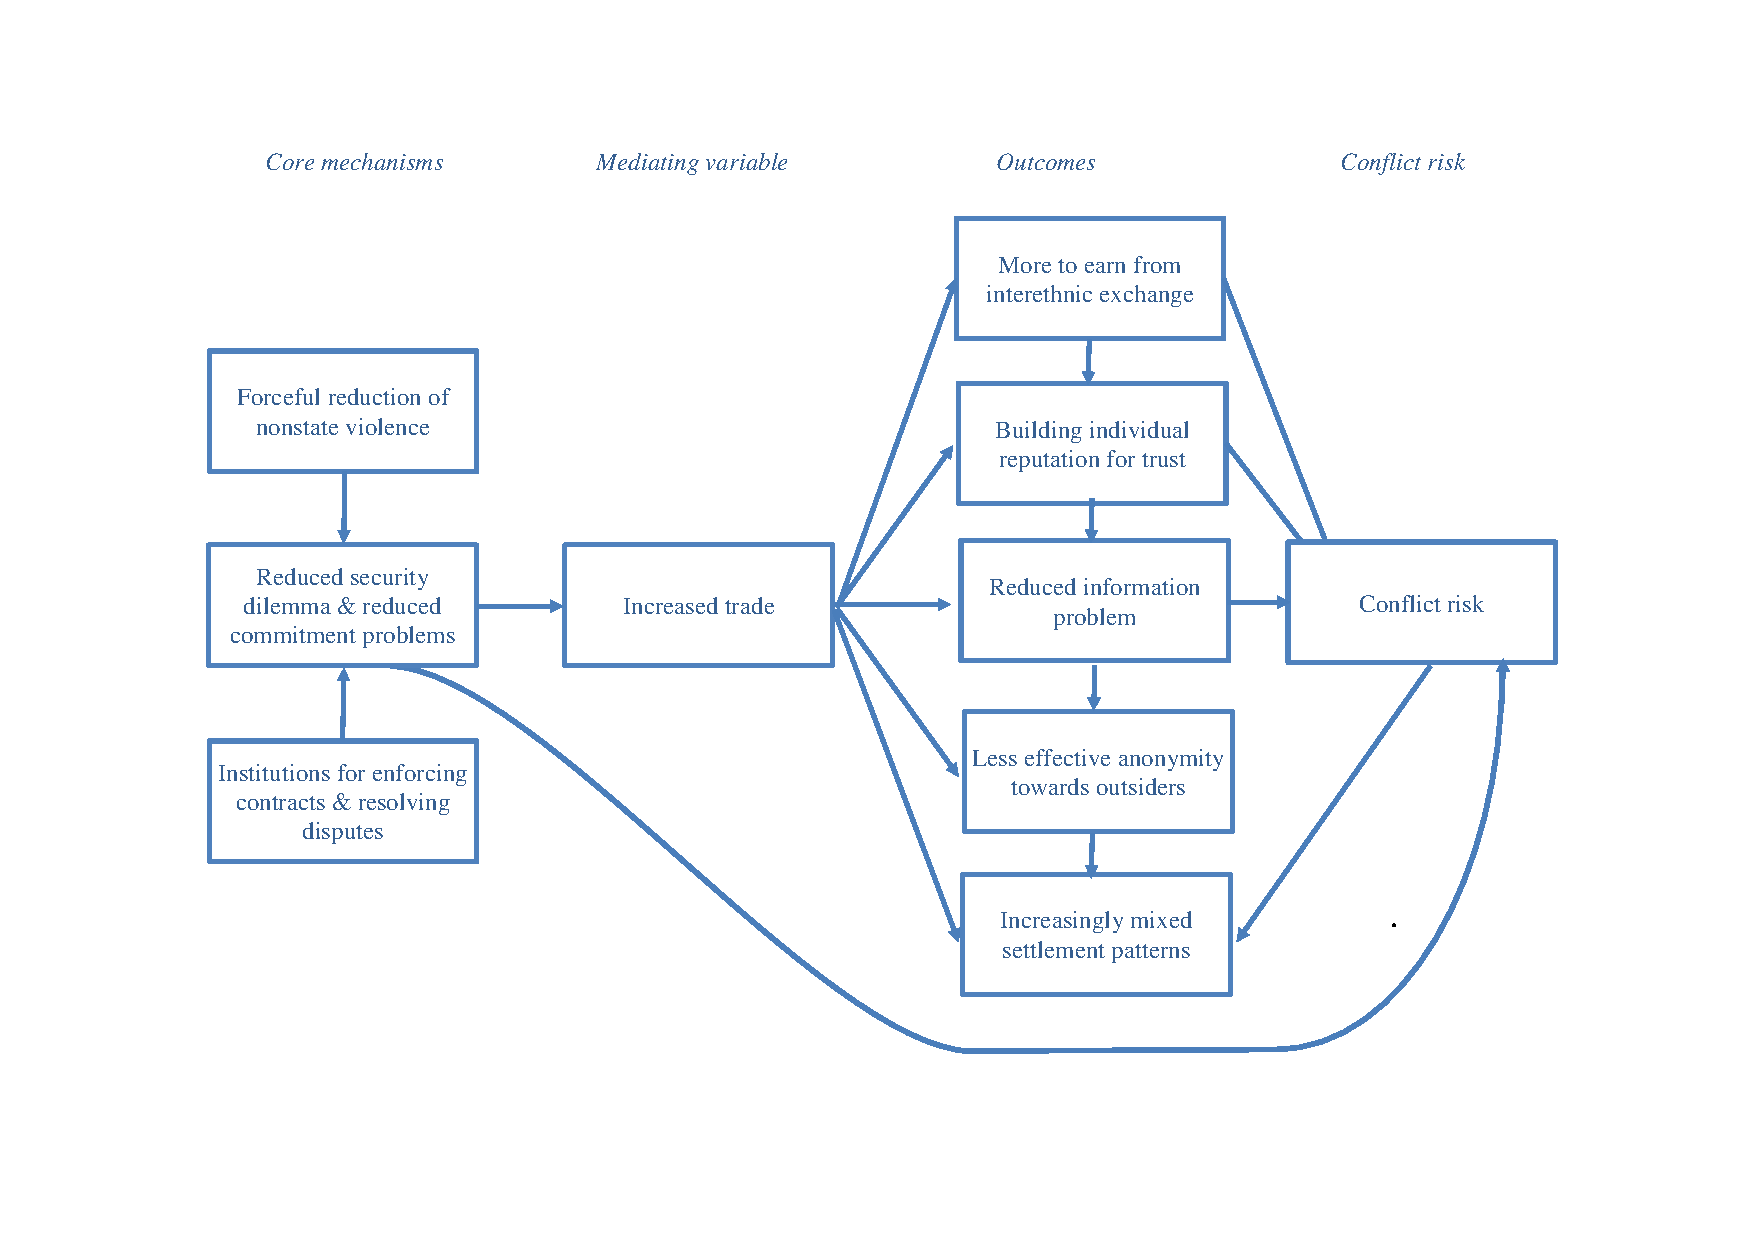
\includegraphics[width=0.8\linewidth]{img/Causal diagram.pdf}
	\caption{Causal diagram}
	\label{causal}
\end{figure}

\section{What lingering effects do precolonial states have today?}

In the postcolonial period, we expect there to be a general reduction in
communal violence over time, in all areas, as they are now under the control of
a state that tries to assert a monopoly of violence. Similarly to how
precolonial states have reduced communal violence, the (national) state resolves
the security dilemma, commitment issues, and gradually reduce information
problems over time. However, there are a few key differences. We assume that
postcolonial states are generally more multiethnic than precolonial states, due
to their larger average size. Simultaneously (especially in the initial period
after indipendence) they are relatively lacking the capacity to project force
(equally) across its whole territory.\footnote{Keep in mind that unlike a
multiethnic precolonial state like Kanem Bornu, the multiethnic state of Kenya
never used its \textit{own} instruments/institutions of power to establish its
borders, and incorporate its various ethnic groups.} We argue that areas differ
both in their initial level of communal violence (as outlined in the following
paragraph), but also in the rate at which new national governments have been
able to reduce it further.

\subsection{The leftover effect}

Precolonial states were able to solve the security dilemma, commitment issues
and information problems between different communities in the past, setting in
motion virtuous cycles of increased interaction, trade and mixed settlement.
This shifted individual motivations toward long term cooperation and against
defecting/cheating in the short term, leading to a reduction in communal
violence. This reduction should be stable or even improve further with time for
as long as there is a state to uphold order. While in most cases pre-colonial
states were either conquered by other precolonial states or colonisers, even in
the few cases where previously state controlled ares have descended into
statelessness, improvements to the information problem could linger. We argue
that in areas with a history of precolonial statehood there is a `leftover
effect' from its time as an independent state. Because the virtuous cycles that
reduce the information problem over time have been in effect for a relatively
longer period, these areas start at a lower relative level of communal violence
in the postcolonial period. Because the establishment and consolidation of
states is what has had the most direct effect on suppression of raiding and
feuding \citep{Pinker2012}, we argue this is the main avenue through which
precolonial states affect postcolonial levels of communal violence.

% We acknowledge that if in some areas colonization, decolonization, or some
% other upheaval has caused a severe breakdown of the state's (pre-, colonial, or
% postcolonial) ability to solve the security dilemma and commitment issues, the
% relationship between groups could break down and initiate a reverse cycle of
% increasing information problems and decreasing interaction between groups.

\subsection{Ease of integration}

Areas above a certain minimum level of precolonial state presence generally had
some existing institutions (formal or informal) and at the very least vertical
social networks that could be leveraged by colonizers. This facilitated
integration into the framework of colonial administration through systems of
indirect rule, whereby local kings, chiefs and leaders retained their position
at the local level with the colonial power placing itself on top. Even in the
case of more direct forms of rule, in which local rulers were replaced,
integration was probably relatively easier than in places with little to no
experience of statehood. The difference being the relative difficulty of
replacing one hierarchy with another relative to building a hierarchy were non
had previously existed. Additionally, areas outside the reach of precolonial
states were so for a reason. Usually due to the effective distance (in travel
time) from areas able to produce a large enough surplus of food to provision
armies. The relative differences of such conditions had not fundamentally
changed despite European and more modern armies greater ability to reach such
remote areas. Integrating remote areas was still relatively more difficult.
Being better integrated into the colonial administration, and subsequently the
nation state, means that the conflict reducing mechanisms of state, outlined
above, continue to work and even at a higher level (of colony and nation state).

On the other hand, higher levels might be more difficult to integrate directly,
which usually resulted in indirect rule during the colonial era, and more local
autonomy in the post-independent era. This increased local autonomy implies that
such areas are less integrated into modern states than areas of more moderate
levels of precolonial state presence, and thus enjoy less of the modern states
conflict reducing effects. However, they do start at a higher level of
intercommunal interaction (larger `leftover effect'), therefore we argue the
overall effect of precolonial state presence should remain
positive.\footnote{This lack of integration is perhaps evident in the finding
	that such areas are more frequently engaged in violent conflict with the
	central government, especially in areas of high precolonial state
presence far from the capital \citep{Wishman2021}.}

% 	- the lack of statehood and subsequent development I South Sudan
% 	- the lack of a head chief prevented land rights for certain groups in
% 	Darfur, causing trouble when ecological changes forced these groups to
% 	stay longer on others’ lands (as they had no land on their own)

\subsection{Local institutions}

Whether formal or informal, or considered part of indirect rule or not,
precolonial states often left behind institutions in the territories they ruled
\citep{Wig2016, Wig2018}. These institutions should generally be more closely
tailored to local conditions than ones created by colonial administration or an
often remote modern state. By being aware and understanding of local traditions,
customs and culture, such institutions might also prove more effective.
Precolonial states may for example have left specific mediation mechanisms such
as councils or courts for dealing with potential triggers that exist between two
communities. Additionally, by tying agreements to its own institutions,
the breaking of which would jeopardize the institutions themselves or, if tied
to formal (though not necessarily state recognized) institutions,
contract-breaking would require that the very same institution overturn its
own previous decisions. Such institutions make inheritor groups more credible
partners \citep{Wig2018}.

% Joking relations an example of this?

A more general institution that frequently transfer from precolonial states into
the postcolonial period is leadership. Sometimes they were officially
incorporated as part of the state apparatus (as in the case of Rwanda [DOUBLE
CHECK]), sometimes recognised as official ceremonial leader or at times not
recognised by the state at all. Nevertheless leaders can influence the level of
communal violence in at least two ways. Leaders occupy a unique role that
allow them to act mediators. Both preventing conflicts from escalating to
violence and help bring an end violence once it is a fact. Even ceremonial
leaders have acted as key mediators in national level events as in the case of
the Mogho Naba, who played a key role in brokering the return of civilian rule to
Burkina Faso following a military coup in 2015
(\href{https://www.bbc.com/news/world-africa-34340704}{BBC}). Leaders are also
uniquely placed to make more credible commitments as they are better placed to
prevent and punish potential spoilers \citep{Wig2016}.


\subsection{Economic development?}

Better integration with colonial administration and national state could give
precolonial state ares a competitive edge relative to other areas when it comes
to developmental projects and priority from the government. If so that should be
reflected in higher levels of economic development, which is famously linked to
lower levels of conflict. However, this relationship could have been turned on
its head by the "reversal of fortunes" \citep{Acemoglu_2002}. Additionally,
finding accurate measures of subnational (or even national) economic development
is a while can of worms.

\section{Observable implications}

% But, do we expect (pre-colonial) states to increase ICP or to replace it?
% Replace within the PCS-territory and strengthen ICP with outside groups?
% I am leaning towards replacing on both counts

\subsection{Communal violence}

Based on the theoretical discussion our main theoretical expectation is an
inverse relationship between precolonial state presence and communal violence.
In other words, areas that have spent more time as part of a precolonial state,
should experience fewer instances of communal violence. Additionally, areas more
thoroughly under the control of a precolonial state should experience relatively
fewer instances of communal violence than areas closer to the periphery of the
precolonial state's territory. Because the theory only speaks to horizontal
conflicts between different groups we do not expect this relationship to hold
for other (vertical) types of conflict, even other forms of non-state violence. 

\subsection{Mixed settlement}

The causal relationship we suggest implies that there is a positive feedback
loop running between less communal violence and more mixed settlement. On the
face of it, it might seem counter intuitive to expect less communal violence in
areas with more mixed settlement. And that intuition is right. In a setting of
mixed settlement there are a lot more potential triggers to conflict as people
are interacting more frequently, simply as a consequence of proximity.  This is
precisely why communities tend to cluster [SOURCE], and we argue, especially so
when settling outside any state umbrella.

If the relationship between precolonial state presence and communal violence
follows the causal mechanisms in Figure \ref{causal}, there should be evidence
of more mixed settlements in precolonial state areas. While in areas brought under
the state umbrella by colonizers or the modern state, we expect ethnic groups to
live in clearly separated clusters. In order to maximise intragroup cohesion,
necessary for IGP to function.

\subsection{Interethnic trust}

The hypothesised increased interethnic interaction and longer periods of
stability between ethnic groups within precolonial state areas should over time
lead to a relative increase in trust toward other groups. While the increased
interaction only happens among the groups within the precolonial state territory
and neighboring communities, these groups are also likely to be the reference
point for people when asked about trust in non-coethnics.

\subsection{Norms of hospitality and conformism in nonstate societies?}

% Is this observable?
% Does this belong under how non-state groups handle stuff?

This creates cultures that encourage nosiness in coethnics affairs, and norms of
thick-skinedness, extreme self-restraint, generosity, hospitality and politeness
towards outsiders\footnote{Thus the first section of the main text Hávámal on
	Norse norms, literally ‘the guest’s section’ (Gestaþáttr) of Hávamál
	contains maxims allegedly given by the head deity Odin to men for proper
	conduct in a nonstate society inducing almost sacred norms of
hospitality and reciprocity towards stranger guests, but also patience and
cautiousness on behalf of the visitor.}, and strongly discourage hot-headedness.
In the words of \citet[37]{Colson1974} cited in \citep[199]{Cohen2004} ‘people
live in what appears to be a Rousseauian paradise because they take a Hobbesian
view of their situation…’ going out of their way to avoid those single acts of
aggression they fear will cause long spirals of violence. However, as the strong
emphasis on norms of ‘niceness’ towards outsiders in peacetime reflects, these
societies are found to be much less effective at containing violence once
cross-ethnic disputes occur as the failure to retaliate violently would reduce
the credibility of this deterrent strategy \citep[723f]{Fearon_1996}.

% Pinker og høfflighet i sørstatene kontra øst-kysten, kan vi knytte det til
% frykten for at det skal eskalere til gruppe konflikt


\subsection{Stronger effect of PCS presence in British colonies?}

If the assumption that the British to a larger degree ruled their colonies
through indirect rule than other colonisers, then according to our hypothesised
ease of integration and local institutions mechanisms should work better in such
areas. However, this difference in colonial strategy is often exaggerated and
stems more from different official aims than form any real difference in de
facto policy on the ground.

\section{Research design}
\subsection{Main analysis}
 
Our main independent variable of interest, our explanatory variable
is time invariant. This means that we are limited to doing a cross sectional
analysis. If we were to attempt to panel data analysis we would essentially be repeating the
same experiment multiple times with observations that are wrongly assumed to be
independent of each other. 
% Opportunity to take down other recent papers who "solve" this by interacting
% their variable with something that varies (only slightly) over time.
Because our inquiry is spatial in nature we use 1\degree by 1\degree grid cells,
using the PRIO-grid id's and corresponding R-package. Using such a grid cell
aproach has the benefit of avoiding any potential bias introduced by using, for
example, administrative units that might be derived from precolonial borders.

Similarly, the treatment is assigned far ahead of measuring its effects which
exposes potential posttreatment bias. This means that in selecting control
variables we have to weigh the potential for introducing posttreatment bias
against the potential for omitted variable bias. 

For the baseline models we use only geographical controls that should avoid post
treatment bias. While for the extended controls we include population density in
1600 and distance to borders. 1600 should be far enough back in time to be
before the establishment of most of, although not all, of the precolonial states
in the data, and thus also avoid post treatment bias. This measure is however
partly based on interpolation back in time, and so is excluded from the baseline
model out of caution. 

\subsubsection{Dependent variable}

Our dependent variable is communal violence events per grid cell in the
1946-2020 period, as captured by the 'Organizational level 3' variable from the
UCDP Georeferenced Event Dataset (GED) and corresponding UCDP Non-state conflict
dataset. This corresponds to events in which conflicts between 'informally
organized groups' surpass a yearly threshold of 25 battle-related deaths in a
year, and is meant to capture 'communal conflicts'.

\subsubsection{Independent variable}

The main explanatory variable is precolonial state presence, as measured by the
main aggregated variable of the Georeferenced International Systems Data
(Geo-ISD) \citep{Wishman2021}. Based on hundreds of maps from the period
1800-1914, complimented by historical atlases compiled by later historians, it
measures state presence by counting how many maps places any given state from
the ISDv2 within each PRIO-grid cell per year.  This captures the dynamism of
borders. Both within a given year, assuming that the more maps agree that a
state controlled an area the more real this control was, and across time, as
state rose and fell some areas were under state control for more years than
others. The definition of state that is used is derived from the ISDv2
\citep{Butcher2020}. The ISD records sovereign states across the 1814-2016
period, defined as political entity with a population of at least 10,000,
autonomy over a specific territory and sovereignty that is either uncontested or
acknowledged by relevant international actors \citep{Butcher2020}.\footnote{For
a more in depth discussion of the definition of and criteria for statehood that
the ISD is based on, see \citet{Butcher2017}.} We use the measure of state
presence that includes interpolated years from historical atlases (shapes are
drawn across all years in which historical atlases depicted borders over a range
of years). For a further discussion of the precolonial state presence measure
see \citet{Wishman2021}. 

\subsubsection{Controls}

We control for how mountainous a grid cell is on average because this could
influence state building, by making it more difficult for people to leave
the oppression of a state, and by providing natural defences. At the same time
mountains affect population density negatively which affects both state
building and conflict events. Generally speaking fighting occurs where there are
at least some people. Lastly, mountainous terrain can be more difficult for a
modern state to reach, and so the same mechanisms we describe for the state
ability to repress communal violence might work independent of precolonial state
presence. 

% Could actually be a matter of catching pockets of low state presence within
% otherwise "stated" territory.

Similarly, access to water is a key ingredient of state building, while it also
proxies population densisty to some degree (people tend to live near water).
Additionally, communal conflicts could erupt over access to water (either
drinking water, for people or herds, or for irrigation).

We also included a measure of how much of
a cell is barren, as a proxy for population density. People generally do not
live in barren areas, and so we do not expect a lot of fighting there. At the
same time we do not expect states to proliferate in barren areas.

The mean distance to coast of each cell could be positively correlated with
state building and economic development. The latter of which is expected to
reduce the risk of conflict.

As already mentioned, population density (log) predicts statehood because states
need a certain level of population density in order to form. At the same time
there are a great deal of grid cells on the African continent that are without
population and we expect very little fighting to occur in these. The data was
source from the Maddison project.

All controls except population density are sourced from the PRIO Grid project.

\subsection{Settlement patterns}

Using the SIDE data, which provides high resolution data on ethnic group
settlement patterns, we hope to do a "proper" analysis using this data, but the
non-random sample of countries for which the data is available is a problem. We
might be stuck with a handful of within country analyses.

\subsection{Afrobarometer on trust}

We have got a lot of geocoded Afrobarometer questions we hope will allow us to
"triangulate" our results and proposed mechanisms further, although we have not
yet gotten started on this, apart from manually correcting a lot of geocoding
errors (big thanks to Ole Magnus).

\section{Preliminary Results}

% Move current results to appendix and present non-climate models as main
% results.

Preliminary results look solid. The results hold for just about any model
specification we have tried. We include in the appendix one that did not. When
including controls for temperature and precipitation the effect of precolonial
states disappears for the model using the square root transformation. However,
when running the same regression after excluding cells with no population,
results are once again as expected.

\begin{figure}[htpb]
	\centering
	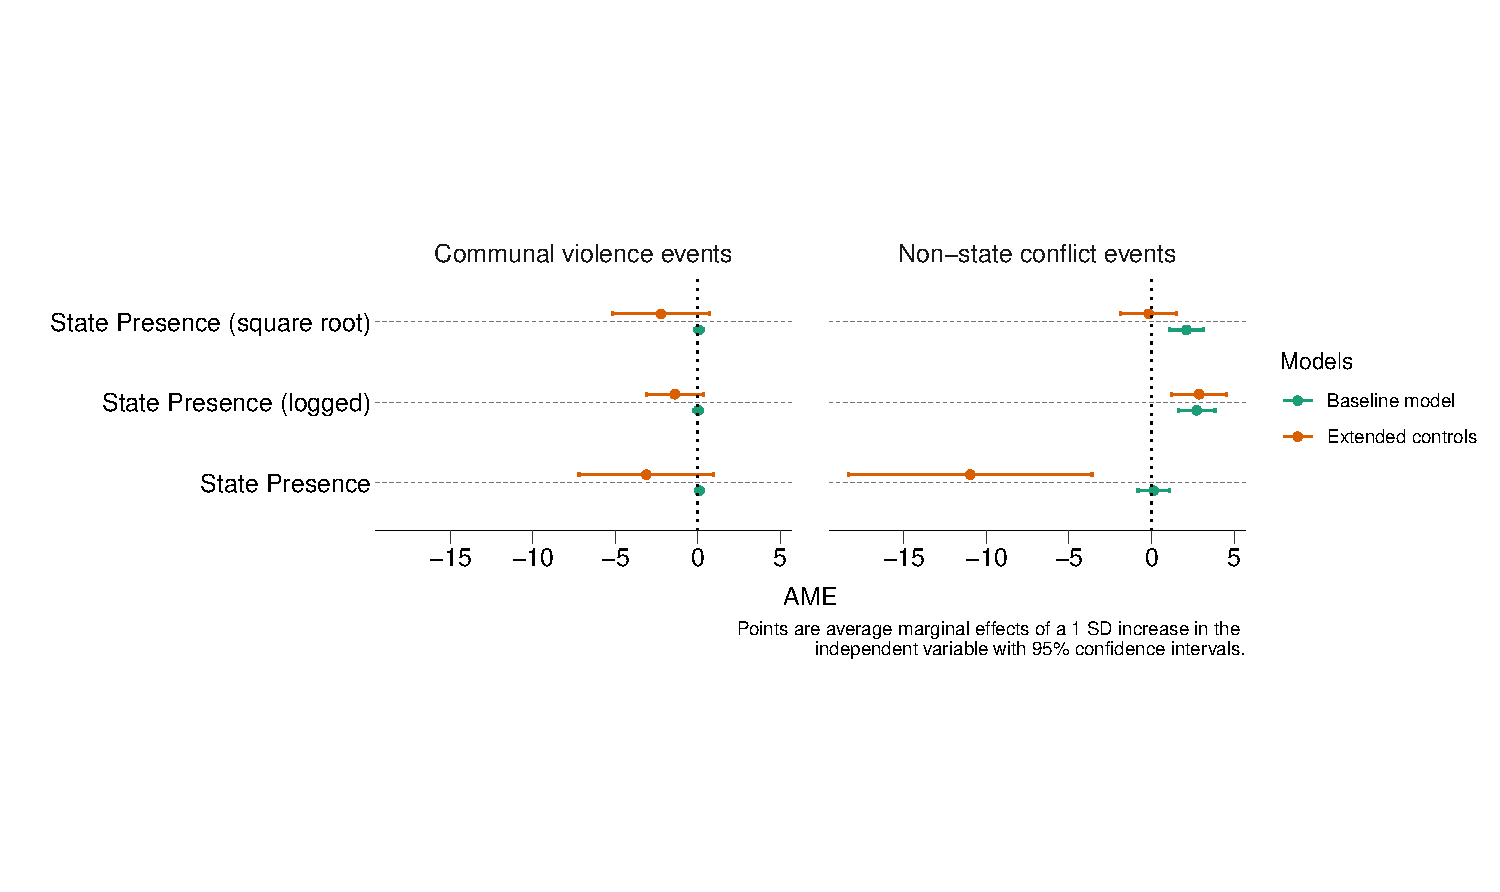
\includegraphics[width=1\linewidth]{../R/Output/CommunalViolenceMargins.pdf}
	\caption{Marginal effects of state presence (sqrt)}
	\label{margins}
\end{figure}

% Change to logit/probit or basian? Chance of any event?


\begin{sidewaystable}
\begin{center}
\scalebox{0.9}{
\begin{tabular}{l c c c c}
\toprule
 & Baseline & North Africa & Population density & Distance
		     to international boundary \\
\midrule
Mountainous terrain                   & $1.92^{***}$ & $1.99^{***}$  & $2.21^{***}$ & $2.29^{***}$ \\
                                      & $(0.54)$     & $(0.53)$      & $(0.48)$     & $(0.48)$     \\
Water (\%)                            & $0.02$       & $0.01$        & $0.04^{**}$  & $0.04^{**}$  \\
                                      & $(0.01)$     & $(0.01)$      & $(0.01)$     & $(0.01)$     \\
Barren (\%)                           & $-0.01^{*}$  & $-0.01$       & $0.00$       & $0.01$       \\
                                      & $(0.01)$     & $(0.01)$      & $(0.01)$     & $(0.01)$     \\
Distance to coast (log)               & $0.23^{***}$ & $0.21^{**}$   & $0.35^{***}$ & $0.36^{***}$ \\
                                      & $(0.06)$     & $(0.06)$      & $(0.07)$     & $(0.07)$     \\
Land not suited for pastorial herding & $0.34$       & $0.08$        & $-0.42$      & $0.09$       \\
                                      & $(0.49)$     & $(0.48)$      & $(0.45)$     & $(0.45)$     \\
North Africa                          &              & $-1.41^{***}$ & $-0.37$      & $-0.38$      \\
                                      &              & $(0.43)$      & $(0.39)$     & $(0.39)$     \\
Population density (log)              &              &               & $1.96^{***}$ & $1.95^{***}$ \\
                                      &              &               & $(0.20)$     & $(0.20)$     \\
Distance to border (log)              &              &               &              & $-0.01$      \\
                                      &              &               &              & $(0.12)$     \\
Precolonial state presence (sqrt)     & $0.07^{*}$   & $0.09^{**}$   & $-0.09^{**}$ & $-0.07^{*}$  \\
                                      & $(0.03)$     & $(0.03)$      & $(0.03)$     & $(0.03)$     \\
\midrule
AIC                                   & $3263.42$    & $3257.57$     & $3185.90$    & $3191.01$    \\
BIC                                   & $3320.68$    & $3322.00$     & $3257.48$    & $3269.75$    \\
Log Likelihood                        & $-1623.71$   & $-1619.79$    & $-1582.95$   & $-1584.50$   \\
Deviance                              & $481.55$     & $483.48$      & $504.81$     & $504.20$     \\
Num. obs.                             & $9492$       & $9492$        & $9492$       & $9492$       \\
\bottomrule
\multicolumn{5}{l}{\scriptsize{$^{***}p<0.001$; $^{**}p<0.01$; $^{*}p<0.05$; $^{\cdot}p<0.1$}}
\end{tabular}
}
\caption{Communal violence events}
\label{org3}
\end{center}
\end{sidewaystable}



\begin{sidewaystable}
\begin{center}
\scalebox{1}{
\begin{tabular}{l c c c c}
\hline
 & Baseline & North Africa & Population density & Distance
		     to international boundary \\
\hline
Mountainous terrain               & $1.88^{***}$  & $1.89^{***}$  & $1.73^{***}$  & $1.74^{***}$  \\
                                  & $(0.24)$      & $(0.24)$      & $(0.23)$      & $(0.23)$      \\
Water (\%)                        & $0.00$        & $0.00$        & $-0.00$       & $0.00$        \\
                                  & $(0.01)$      & $(0.01)$      & $(0.01)$      & $(0.01)$      \\
Barren (\%)                       & $-0.03^{***}$ & $-0.03^{***}$ & $-0.02^{***}$ & $-0.02^{***}$ \\
                                  & $(0.00)$      & $(0.00)$      & $(0.00)$      & $(0.00)$      \\
Population density (log)          &               &               & $1.21^{***}$  & $1.20^{***}$  \\
                                  &               &               & $(0.09)$      & $(0.09)$      \\
Precolonial state presence (sqrt) & $0.07^{***}$  & $0.07^{***}$  & $-0.03^{*}$   & $-0.03^{*}$   \\
                                  & $(0.01)$      & $(0.01)$      & $(0.01)$      & $(0.01)$      \\
\hline
AIC                               & $14603.42$    & $14605.30$    & $14455.47$    & $14456.71$    \\
BIC                               & $14653.53$    & $14662.57$    & $14519.90$    & $14528.30$    \\
Log Likelihood                    & $-7294.71$    & $-7294.65$    & $-7218.74$    & $-7218.36$    \\
Deviance                          & $2412.91$     & $2412.85$     & $2439.51$     & $2439.59$     \\
Num. obs.                         & $9492$        & $9492$        & $9492$        & $9492$        \\
\hline
\multicolumn{5}{l}{\scriptsize{$^{***}p<0.001$; $^{**}p<0.01$; $^{*}p<0.05$; $^{\cdot}p<0.1$}}
\end{tabular}
}
\caption{Non-state conflict events}
\label{non_state}
\end{center}
\end{sidewaystable}


\pagebreak

\bibliographystyle{agsm}
\bibliography{../lib.bib}

\pagebreak

\section{Appendix}


\begin{sidewaystable}
\begin{center}
\scalebox{1}{
\begin{tabular}{l c c c c c c}
\hline
 & Baseline & Extended Controls & Climate & Baseline & Extended Controls & Climate \\
\hline
Precolonial state presence (log)  & $0.02$        & $-0.32^{***}$  & $-0.23^{**}$  &               &               &               \\
                                  & $(0.08)$      & $(0.08)$       & $(0.08)$      &               &               &               \\
Mountainous terrain               & $1.83^{**}$   & $1.72^{***}$   & $3.55^{***}$  & $2.26^{***}$  & $1.95^{***}$  & $2.98^{***}$  \\
                                  & $(0.56)$      & $(0.51)$       & $(0.55)$      & $(0.56)$      & $(0.51)$      & $(0.56)$      \\
Water (\%)                        & $-0.04^{***}$ & $-0.03^{**}$   & $-0.04^{**}$  & $-0.04^{***}$ & $-0.03^{**}$  & $-0.05^{***}$ \\
                                  & $(0.01)$      & $(0.01)$       & $(0.01)$      & $(0.01)$      & $(0.01)$      & $(0.01)$      \\
Barren (\%)                       & $-0.03^{***}$ & $-0.00$        & $-0.00$       & $-0.02^{***}$ & $-0.00$       & $-0.00$       \\
                                  & $(0.00)$      & $(0.00)$       & $(0.00)$      & $(0.00)$      & $(0.00)$      & $(0.00)$      \\
Distance to coast                 & $-0.00$       & $0.00^{\cdot}$ & $0.00$        & $-0.00$       & $0.00$        & $-0.00$       \\
                                  & $(0.00)$      & $(0.00)$       & $(0.00)$      & $(0.00)$      & $(0.00)$      & $(0.00)$      \\
Population density (log)          &               & $1.91^{***}$   & $1.99^{***}$  &               & $2.03^{***}$  & $1.94^{***}$  \\
                                  &               & $(0.20)$       & $(0.21)$      &               & $(0.20)$      & $(0.21)$      \\
Distance to border                &               & $-0.00$        & $-0.00$       &               & $-0.00$       & $0.00$        \\
                                  &               & $(0.00)$       & $(0.00)$      &               & $(0.00)$      & $(0.00)$      \\
Temperature (SD)                  &               &                & $0.07$        &               &               & $0.25$        \\
                                  &               &                & $(0.41)$      &               &               & $(0.42)$      \\
Temperature (mean)                &               &                & $0.24^{***}$  &               &               & $0.21^{***}$  \\
                                  &               &                & $(0.04)$      &               &               & $(0.04)$      \\
Precipitation (SD)                &               &                & $0.05^{***}$  &               &               & $0.01$        \\
                                  &               &                & $(0.01)$      &               &               & $(0.01)$      \\
Precipitation (mean)              &               &                & $-0.01^{***}$ &               &               & $-0.00$       \\
                                  &               &                & $(0.00)$      &               &               & $(0.00)$      \\
Precolonial state presence (sqrt) &               &                &               & $0.02$        & $-0.13^{***}$ & $0.00$        \\
                                  &               &                &               & $(0.03)$      & $(0.03)$      & $(0.03)$      \\
\hline
AIC                               & $3331.33$     & $3259.48$      & $3250.94$     & $3327.30$     & $3260.05$     & $3255.51$     \\
BIC                               & $3382.14$     & $3324.80$      & $3345.25$     & $3378.11$     & $3325.36$     & $3349.82$     \\
Log Likelihood                    & $-1658.66$    & $-1620.74$     & $-1612.47$    & $-1656.65$    & $-1621.02$    & $-1614.76$    \\
Deviance                          & $484.10$      & $505.10$       & $510.28$      & $485.35$      & $503.49$      & $506.47$      \\
Num. obs.                         & $10492$       & $10482$        & $10453$       & $10492$       & $10482$       & $10453$       \\
\hline
\multicolumn{7}{l}{\scriptsize{$^{***}p<0.001$; $^{**}p<0.01$; $^{*}p<0.05$; $^{\cdot}p<0.1$}}
\end{tabular}
}
\caption{Communal violence events}
\label{org3Full}
\end{center}
\end{sidewaystable}



\begin{sidewaystable}
\begin{center}
\scalebox{1}{
\begin{tabular}{l c c c c c c}
\hline
 & Baseline & Extended Controls & Climate & Baseline & Extended Controls & Climate \\
\hline
Precolonial state presence (log)  & $0.20^{***}$  & $0.14^{***}$  & $0.15^{***}$  &               &               &               \\
                                  & $(0.04)$      & $(0.04)$      & $(0.04)$      &               &               &               \\
Mountainous terrain               & $2.07^{***}$  & $2.30^{***}$  & $2.28^{***}$  & $1.86^{***}$  & $2.00^{***}$  & $1.80^{***}$  \\
                                  & $(0.25)$      & $(0.24)$      & $(0.26)$      & $(0.25)$      & $(0.24)$      & $(0.26)$      \\
Water (\%)                        & $0.02^{***}$  & $0.02^{***}$  & $0.02^{***}$  & $0.02^{***}$  & $0.02^{***}$  & $0.02^{***}$  \\
                                  & $(0.00)$      & $(0.00)$      & $(0.00)$      & $(0.00)$      & $(0.00)$      & $(0.00)$      \\
Barren (\%)                       & $-0.03^{***}$ & $-0.02^{***}$ & $-0.02^{***}$ & $-0.03^{***}$ & $-0.02^{***}$ & $-0.02^{***}$ \\
                                  & $(0.00)$      & $(0.00)$      & $(0.00)$      & $(0.00)$      & $(0.00)$      & $(0.00)$      \\
Distance to coast                 & $-0.00^{**}$  & $-0.00$       & $0.00$        & $-0.00^{**}$  & $-0.00$       & $0.00$        \\
                                  & $(0.00)$      & $(0.00)$      & $(0.00)$      & $(0.00)$      & $(0.00)$      & $(0.00)$      \\
Population density (log)          &               & $1.06^{***}$  & $1.17^{***}$  &               & $1.11^{***}$  & $1.24^{***}$  \\
                                  &               & $(0.09)$      & $(0.10)$      &               & $(0.09)$      & $(0.10)$      \\
Distance to border                &               & $-0.00$       & $-0.00$       &               & $0.00$        & $-0.00$       \\
                                  &               & $(0.00)$      & $(0.00)$      &               & $(0.00)$      & $(0.00)$      \\
Temperature (SD)                  &               &               & $0.16$        &               &               & $0.19$        \\
                                  &               &               & $(0.20)$      &               &               & $(0.20)$      \\
Temperature (mean)                &               &               & $-0.03$       &               &               & $-0.05^{**}$  \\
                                  &               &               & $(0.02)$      &               &               & $(0.02)$      \\
Precipitation (SD)                &               &               & $0.01$        &               &               & $0.01$        \\
                                  &               &               & $(0.01)$      &               &               & $(0.01)$      \\
Precipitation (mean)              &               &               & $-0.00^{***}$ &               &               & $-0.00^{**}$  \\
                                  &               &               & $(0.00)$      &               &               & $(0.00)$      \\
Precolonial state presence (sqrt) &               &               &               & $0.06^{***}$  & $-0.00$       & $-0.01$       \\
                                  &               &               &               & $(0.01)$      & $(0.01)$      & $(0.01)$      \\
\hline
AIC                               & $14248.68$    & $14125.84$    & $14085.64$    & $14260.63$    & $14135.40$    & $14094.60$    \\
BIC                               & $14299.48$    & $14191.16$    & $14179.96$    & $14311.44$    & $14200.71$    & $14188.91$    \\
Log Likelihood                    & $-7117.34$    & $-7053.92$    & $-7029.82$    & $-7123.31$    & $-7058.70$    & $-7034.30$    \\
Deviance                          & $2341.13$     & $2364.66$     & $2363.01$     & $2338.65$     & $2363.76$     & $2361.71$     \\
Num. obs.                         & $10492$       & $10482$       & $10453$       & $10492$       & $10482$       & $10453$       \\
\hline
\multicolumn{7}{l}{\scriptsize{$^{***}p<0.001$; $^{**}p<0.01$; $^{*}p<0.05$; $^{\cdot}p<0.1$}}
\end{tabular}
}
\caption{Non-state conflict events}
\label{non_stateFull}
\end{center}
\end{sidewaystable}


\end{document}
	
